%\documentclass{beamer} 

\documentclass[aspectratio=169,compress]{beamer}
\mode<presentation> 

\usepackage{color}

\usetheme{Warsaw}
\usepackage{beamerouterthememiniframes} % Para los puntitos 
\setbeamertemplate{footline}[page number]{} % Pone el n\'umero de Diapositiva
\setcounter{tocdepth}{1} 

% Requerido para la entrada con acentos
\usepackage[utf8x]{inputenc}
\usepackage[T1]{fontenc}
\usepackage[spanish]{babel}

\usepackage{listings} % Para los Codigos y el problema de BEAMER que no

% include packages
% Libreria que permite dividir las diapositivas en multipes columans
\usepackage{multicol}
% Libreria que permite la insercion de imagenes
\usepackage{graphicx}
%\usepackage[dvips]{graphicx}
% Soporta imagenes EPS
\usepackage{epsfig}

\usepackage{verbatim}
\usepackage{moreverb}
\let\verbatiminput=\verbatimtabinput



     
%%%%%%%%%%%%%%%%%%%%%%%%%%%%%%%%%%%%%%%%%%%%%%%%%%%%%%%%%%%%%%%%%%%%%%%%%%%%%%%%%%%%%%%%%%
%%%%%%%%%%%%%%%%%%%%%%%%%%%%%% Title Page Info %%%%%%%%%%%%%%%%%%%%%%%%%%%%%%%%%%%%%%%%%%%
%%%%%%%%%%%%%%%%%%%%%%%%%%%%%%%%%%%%%%%%%%%%%%%%%%%%%%%%%%%%%%%%%%%%%%%%%%%%%%%%%%%%%%%%%%

\title{Herramientas Open Source para Creación de Reportes Técnicos y Científicos}
%\subtitle{The Beamer Class}
\author{Dr. Marco Aurelio Nu\~no-Maganda}
\institute{\\ 
Universidad Politecnica de Victoria \\ 
mnunom@upv.edu.mx \vspace{.25cm} }
\date{27 de OCTUBRE de 2011}

\lstset{basicstyle=\tiny\ttfamily,framerule=4cm}
\begin{document}

\newcommand{\archivolatex}[1]{
	\tiny
	\verbatiminput{#1} 
}

\frame{
	
	\begin{titlepage}
	\end{titlepage}
	
}

\frame{\frametitle{Contenido del Curso}\tableofcontents}

\section{\LaTeX}
\subsection{Fundamentos de \LaTeX}
\frame{
	\frametitle{Introduccion}	
	Tipos de procesadores de texto
	
	\begin{itemize}
		\item WYSIWYG (What You See Is [all] What You Get)
	
	\begin{itemize}
		\item Microsoft Word
		\item Corel WordPerfect
		\item OpenOffice Writer (LibreOffice Writer)
	\end{itemize}
	\item Sistemas de Fotocomposicion Automatizados (Por ejemplo: \LaTeX)
	
\begin{itemize}
	\item Se crea el documento a partir de un ``código'' fuente almacenado en cualquier archivo de texto. 
\end{itemize}
\end{itemize}

Ventajas:
\begin{itemize}	
	\item Es gratuito y abierto (Open Soruce). 
	\item Existen versiones para equipos con pocos recursos 
\end{itemize}
Desventajas:
\begin{itemize}
	\item La curva de aprendizaje es mas lenta.
\end{itemize}


}


  \frame
  {
    \frametitle{Características de un Sistema de Fotocomposición}

    \begin{itemize}
    \item \LaTeX\ \ es un sistema de defición de documentos de alta calidad
    \item Se puede utilizar para cualquier tipo de documento, aunque es especialmente útil para documentos complejos (libros, tesis, reportes técnicos, artículos científicos, reportes de proyecto final, etc).
    \item \textbf{¡No es un Procesador de Textos¡} - es un lenguaje de definición de documentos con reglas bien establecidas. 
    \item Se requieren 3 elementos básicos
	    \begin{enumerate}
		    \item Editor de texto
		    \item Compilador
		    \item Programa visor de tipo de archivo de salida (PDF, PS, DVI)
	    \end{enumerate}
    \end{itemize}
  }

  \frame
  {
    \frametitle{Herramientas Requediras para trabajar con Latex}
    Ejemplos de Herramientas (Open Source) requeridas para trabajar con \LaTeX:
    \begin{itemize}
    \item Editores de texto: gedit (recomendado), emacs, bluefish, nano, jEdit, Komod, SciTe, Vim, Pico, etc
    \item Compiladores:
	    \begin{itemize}
	    \item pdflatex - genera archivos de salida en formato PDF
	    \item latex - genera archivos en formado DVI 
	    \end{itemize}
    \item Visualizador de archivos de salida: evince y acroreader para archivos PDF, ghostview para PS, etc. 
    \end{itemize}
  }


\section{Instalación}
\subsection{Múltiples plataformas}
  \frame
  {
    \frametitle{Instalación de Latex}
    En Linux:
    \begin{itemize}
	\item Se recomienda instalar a partir de los repositorios de la distribución de Linux utilizada
	\item Pasos para instalar el compilador usando apt-get (se necesita instalar desde linea de comando):
	    \begin{itemize}
		\item Para instalar el compilador y los diferentes paquetes: \textbf{sudo apt-get install texlive-latex-base}
		\item Para instalar los paquetes necesarios para crear presentaciones: \textbf{sudo apt-get install latex-beamer}
		\item Para instalar el convertidor de latex a RTf: \textbf{sudo apt-get install latex2rtf}
	    \end{itemize}
    \end{itemize}
    En Windows: \url{http://miktex.org/}. 

  }

  \frame
  {
    \frametitle{Características del Lenguaje}
    Datos reelevantes del código:
    \begin{itemize}
	\item Sensible a mayúsculas y minúsculas (principalmente se utilizan minúsculas).
	\item Se deben incluir los paquetes que contengan las características que se desean utilizar.
    \end{itemize}
    Propósitos:
    \begin{itemize}
	\item Permitir al usuario promedio editar libros de alta calidad
	\item Un sistema que generé el mismo documento en cualquier computadora
    \end{itemize}	
  }

%  \section{Compilación de un archivo en \LaTeX}


%\section{Fundamentos}
\subsection{Primer Documento en LATEX}

\frame{
	\frametitle{Primer Documento en \LaTeX}	
	Caracter\'isticas de Sintaxis basica del documento
		\begin{itemize}
			\item Todos los comandos inician con $\backslash$
			\item Existen dos partes principales: 			
\begin{itemize}
%\item X
	\item \textbf{Primera parte: Definici\'on de parametros}. Se definen los parametros y paquetes a utilizar. Al menos se debe especificar el tipo de documento. Para esto se requiere el comando: $\backslash$ documentclass [ \textit{Opciones} ] \{ \textit{Tipo} \} Los valores permitidos para \textit {Tipo} son: 
	
\begin{itemize}
	\item \textit{article}. Se utiliza para elaborar art\'iculos de congresos y revistas especializadas. 
	\item \textit{report}. Se utiliza para crear informes, libros peque\~nos, etc
	\item \textit{book}. Clase para crear libros u documentos a doble cara 
	\item \textit{slide}. Clase basica para diapositivas
	\item \textit{beamer}. Clase avanzada para diapositivas
\end{itemize}

\end{itemize}
		\end{itemize}  	
}


\frame{
	\frametitle{Documento B\'asico}	
  \begin{columns}
  \column {0.4\textwidth}        	
  	Se requieren de ciertos comandos para definir el texo
		\begin{itemize}
			\item \textbf{Segunda parte: Definici\'on del texto del documento}.  En este caso, para el documento mas sencillo se necesitara $\backslash$begin\{document\} y $\backslash$end\{document\}. Todo el texto definido entre estas dos directivas en integrado en el documento. 			
		\end{itemize}
  \column {0.6\textwidth}      	
		\begin{block}{Ejemplo 1}			
		\begin{minipage}{3cm}
			\archivolatex{uno.tex}
 		\end{minipage}
		\end{block}
	 \end{columns}
}

  \frame
  {
    \frametitle{Compilación de un archivo en \LaTeX}

	\begin{itemize}		
	     \item Es necesario abrir una terminal y ejecutar
		\begin{center}
		\textbf{pdflatex <NombreArchivo.tex>}
		\end{center}
		\item Esto genera un archivo de nombre <NombreArchivo.pdf> en el directorio donde está localizado el archivo fuente, para visualizar el archivo resultante es necesario ejecutar:
	\begin{center}
		\textbf{evince <NombreArchivo.pdf>}
	\end{center}
	\end{itemize}		  
}


\frame{
	\frametitle{}	
	Las opciones mas comunes son:
	
\begin{itemize}
	\item El tama\~no de letra. Si no se especifica, por defecto se utiliza un tama\~no de 10pt (Opciones: \textbf{10pt, 11pt, 12pt, .... }) 
	\item El tama\~no del papel: \textbf{a4paper, letterpaper}. 
	\item El numero de columnas. La opci\'on \textbf{twocolumn} permite generar documentos a doble columna.  
	\item El numero de caras del documento. \textbf{oneside, twoside}. Los documentos tipo \textbf{article} y \textbf{report} son a una cara, mientras que \textbf{book} es a dos caras.	
	\begin{block}{Ejemplo de uso}
	$\backslash$documentclass[12pt,letterpaper,oneside]\{article\}
	\end{block}	
\end{itemize}
}

\section{Organizaci\'on}
\subsection{Capítulos, Secciones y Subsecciones}
\frame{
	\frametitle{Secciones y Subsecciones}	
  \begin{columns}
  \column {0.4\textwidth}        	
		Es posible organizar el documento en diferentes secciones. 
		\begin{itemize}
			\item Secciones: 
			\begin{block}{}$\backslash$section\{\textit{Titulo}\}
			\end{block}
			\item Sub-Secciones: 
			\begin{block}{} $\backslash$subsection\{\textit{Titulo}\}
			\end{block}
			\item Sub-Sub-Secciones: 
			\begin{block}{}$\backslash$subsubsection\{\textit{Titulo}\}
			\end{block}
		\end{itemize}
  \column {0.6\textwidth}      	
		\begin{block}{Ejemplo2}			
		%\includegraphics[scale=0.40]{codigo2.jpg}
			\begin{minipage}{3cm}
				\archivolatex{dos.tex}
 			\end{minipage}
		\end{block}
	 \end{columns}
		
		
		%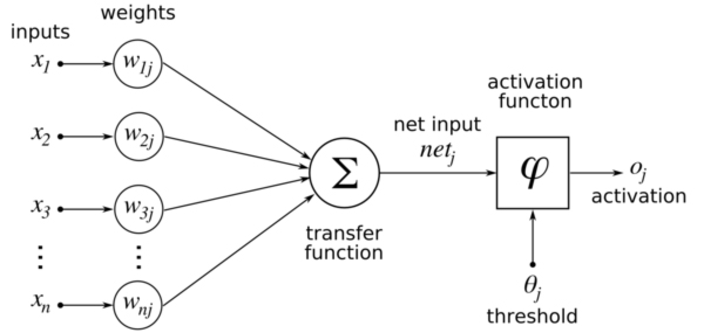
\includegraphics[width=300pt,height=133pt]{NeuronaArtificial.pdf}
		%\pgfimage[height=5cm]{NeuronaArtificial}
		
}

\frame{
	\frametitle{Clase book}	
  \begin{columns}
  \column {0.4\textwidth} 
  Se crea un documento de 3 paginas, donde la primera pagina de cada capitulo queda en Pagina IMPAR
  
  Problema: El titulo del capitulo es ``Chapter''. Cambio para renombrar el nombre del capitulo: definir en el preambulo el siguiente comando:       	
  \begin{block}{}
  $\backslash $
  renewcommand 
  \{$\backslash$chaptername\}
  \{Capitulo\}  
  %
\includegraphics[scale=0.7]{RenameChapter.jpg}
  \end{block}
  %Melle
  \column {0.6\textwidth}      	
		\begin{block}{Ejemplo 3}			
		%\includegraphics[scale=0.40]{codigo3.jpg}
			\begin{minipage}{3cm}
				\archivolatex{tres.tex}
	 		\end{minipage}
		\end{block}
	 \end{columns}
		
		
		%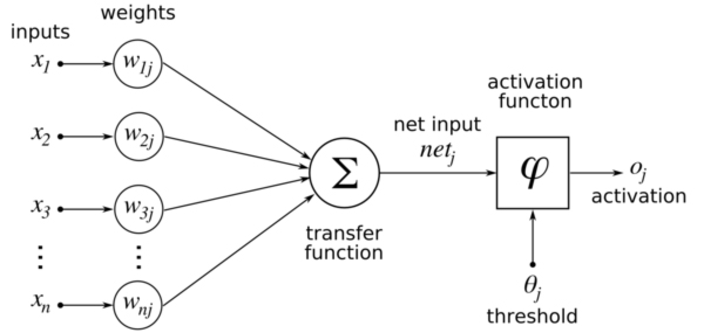
\includegraphics[width=300pt,height=133pt]{NeuronaArtificial.pdf}
		%\pgfimage[height=5cm]{NeuronaArtificial}
		
}

\section{Portadas}
\subsection{Formato Predefinido}
\frame{
	\frametitle{Estilo predefinido por \LaTeX}	
  \begin{columns}
  \column {0.4\textwidth} 
  Se definen en el preambulo los campos globales
  
	\begin{itemize}
		\item $\backslash$title\{\textit{Titulo}\}
		\item $\backslash$author\{\textit{Autor}\}
		\item $\backslash$data\{\textit{Fecha}\}
	\end{itemize}

	Ya en el documento, se utiliza el comando $\backslash$maketitle
 
  \column {0.6\textwidth}    
		\begin{block}{Ejemplo 4}			
		%\includegraphics[scale=0.40]{codigo4.jpg}
			\begin{minipage}{3cm}
				\archivolatex{cuatro.tex}
	 		\end{minipage}

		\end{block}
	 \end{columns}
    	
	

}


\subsection{Pagina de Portada Definida por el Autor}
\frame{
	\frametitle{Estilo predefinido por el Autor}	
  \begin{columns}
  \column {0.4\textwidth} 
  Es posible definir una portada personalizada, con los comandos: \\
  $\backslash$begin\{\ titlepage \} \\
  \% Contenido de la Portada  \\
  $\backslash$end\{\ titlepage \} \\
  \column {0.6\textwidth}    
		\begin{block}{Ejemplo 5}			
%		\includegraphics[scale=0.40]{codigo5.jpg}
			\begin{minipage}{3cm}
% 				\testcodecinco
				\archivolatex{cinco.tex}
	 		\end{minipage}

		\end{block}
	 \end{columns}
}

%\section{TOC}
\subsection{TOC (Table of Contents)}
\frame{
	\frametitle{Tabla de Contenidos}	
  \begin{columns}
  \column {0.4\textwidth} 
  Es posible agregar una tabla de contenidos\\
  \begin{block}{Comando}
  $\backslash$tableofcontents
  \end{block}
  \column {0.6\textwidth}    
		\begin{block}{Ejemplo 6}			
		%\includegraphics[scale=0.40]{codigo6.jpg}
			\begin{minipage}{3cm}
% 				\testcodeseis
				\archivolatex{seis.tex}
	 		\end{minipage}

		
		\end{block}
	 \end{columns}
	
}


\section{Formatos}
\subsection{Formato de Texto}
\frame{
	\frametitle{Acentos y Caracteres Especiales (Método Tradicional)}	
  \begin{columns}
  \column {0.4\textwidth} 	
	Hay algunos caracteres que requieren de secuencias especiales para generarlos para su impresi\'on. 
	
\begin{table}
\begin{center}
\begin{tabular}{cc}
\hline
Caracter & Secuencia \\
\hline
\} & \textbf{$\backslash$\}} \\
\# & \textbf{$\backslash$\#} \\
\$ & \textbf{$\backslash$\$} \\
\& & \textbf{$\backslash$\&} \\
\% & \textbf{$\backslash$\%} \\
Acento (\'a) & \textbf{$\backslash$'a} \\
Tilde  (\~N) & \textbf{$\backslash$(tilde)N} \\
\hline
\hline
\end{tabular}
\end{center}
\end{table}	
	  \column {0.6\textwidth} 
		\begin{block}{Ejemplo 7}			
		%\includegraphics[scale=0.40]{codigo7.jpg}
			\begin{minipage}{3cm}
% 				\testcodesiete
				\archivolatex{siete.tex}

	 		\end{minipage}		
		\end{block}
	 \end{columns}
 
}								 

\frame{
	\frametitle{Acentos y Caracteres Especiales (Método Simplificado) }	
  \begin{columns}
  \column {0.4\textwidth} 	
	Es posible introducir directamente caracteres acentuados. Solo es necesario declarar en el preámbulo un conjunto de paquetes que permite tal inserción. 	
	  \column {0.6\textwidth} 
		\begin{block}{Ejemplo 7}			
			\begin{minipage}{3cm}
				\archivolatex{sietea.tex}

	 		\end{minipage}		
		\end{block}
	 \end{columns}
 
}								 
						 
%\subsection{Formato de Texto}
\frame{
	\frametitle{Centrado, Justificado  }	
  \begin{columns}
  \column {0.4\textwidth} 	
		\begin{itemize}
			\item Centrado. $\backslash$begin\{center\} y $\backslash$end\{center\}.
			\item Justificado por Izquierda:  $\backslash$begin\{flushleft\} y $\backslash$end\{flushleft\}. 			
			\item Justificado por Derecha:  $\backslash$begin\{flushright\} y $\backslash$end\{flushright\}. 						
			\end{itemize}
	  \column {0.6\textwidth} 
		\begin{block}{Ejemplo8}			
		%\includegraphics[scale=0.40]{codigo8.jpg}
			\begin{minipage}{3cm}
 	%			\testcodeocho
				\archivolatex{ocho.tex}
	 		\end{minipage}	
		\end{block}
	 \end{columns}
			
}
							 
\frame{
	\frametitle{Tama\~nos y Tipos de letra }	
  \begin{columns}
  \column {0.4\textwidth} 	
  
\begin{itemize}
	\item Fuente Predefinida es \textrm{Roman}, otras fuentes: \textsf{Sans Serif} y\texttt{ Typewriter}. 
	\item Por defecto, el tama\~no es normalsize, pero puede ser cambiarda
	\item El paquete geometry permite definir los margenes del documento.
\end{itemize}
  \column {0.6\textwidth} 	
		\begin{block}{Ejemplo 8A}			
		%\includegraphics[scale=0.40]{codigo7.jpg}
			\begin{minipage}{3cm}
 				%\testcodeochoa
			\archivolatex{ocho_a.tex}	 
		\end{minipage}		
		\end{block}
  
  \end{columns}
}
							 
							 


\subsection{Numeracion y vi\~netas}
\frame{
	\frametitle{Entornos}	
  \begin{columns}
	  \column {0.4\textwidth} 	

	\begin{block}{Lista Elementos}	  
	$\backslash$begin\{itemize\} \\
	$\backslash$item Elemento1 \\
	$\backslash$item Elemento2 \\
	$\backslash$end\{itemize\}.	\\   
	\end{block}

	\begin{block}{Lista Elementos Numerada}	  
	$\backslash$begin\{enumerate\} \\
	$\backslash$item Elemento1 \\
	$\backslash$item Elemento2 \\
	$\backslash$end\{enumerate\}.\\	  
	\end{block}
	
			
	  \column {0.6\textwidth} 
		\begin{block}{Ejemplo 9}			
%		\includegraphics[scale=0.40]{codigo9.jpg}
			\begin{minipage}{3cm}
 				%\testcodenueve
				\archivolatex{nueve.tex}	 
	 		\end{minipage}	

		\end{block}
	 \end{columns}
	
}

\section{Figuras y Tablas}
\subsection{Figuras}
\frame{
	\frametitle{Figuras}	
	  \begin{columns}
	  \column {0.4\textwidth}
	\begin{block}{Sintaxis}	
		\includegraphics[scale=0.25]{SintaxisFigure.jpg}
		\end{block}
	
	\begin{itemize}
	\item \small  Se requiere la libreria \textbf{graphicx}
	\item \tiny  Se utiliza \textit{CAPTION} que permite definir el texto del pie de la figura.
	\item \tiny  Se utiliza \textit{LABEL}, que es una etiqueta que permite hacer referencia a la figura.
	\item \tiny  Se utiliza \textbf{includegraphics} permite definir un archivo de imagen JPEG o PDF.  
\end{itemize} 
	  
	  
	\column {0.6\textwidth} 
		\begin{block}{Ejemplo10}			
%		\includegraphics[scale=0.40]{codigo10.jpg}
			\begin{minipage}{3cm}
% 				\testcodediez
				\archivolatex{diez.tex}	 

	 		\end{minipage}	

		\end{block}
	 \end{columns}

}

\frame{
	\frametitle{Hacer Referencia a Figuras en el Texto}	
	  \begin{columns}	  
	  \column {0.4\textwidth} 
	  Para cada figura se debe definir una etiqueta. Es posible definir
	  una referencia hacia esta etiqueta. 
			\begin{block}{Sintaxis}	
				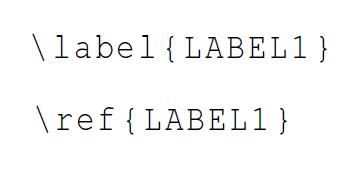
\includegraphics[scale=0.25]{Sintaxis_Label_REF.jpg}
				\end{block}
	\column {0.6\textwidth} 
		\begin{block}{Ejemplo11}			
		%\includegraphics[scale=0.40]{codigo11.jpg}
			\begin{minipage}{3cm}
% 				\testcodeonce
				\archivolatex{once.tex} 
	 		\end{minipage}	

		\end{block}
	 \end{columns}

}

%\section{Tablas}
\subsection{Tablas}
\frame{
	\frametitle{Definicion de Tablas}	
	  \begin{columns}
	  \column {0.4\textwidth} 

	\begin{block}{Sintaxis Table}	
		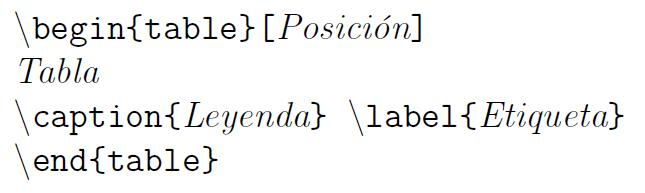
\includegraphics[scale=0.25]{SintaxisTable.jpg}
		\end{block}
	\begin{block}{Sintaxis de Tabular}	
		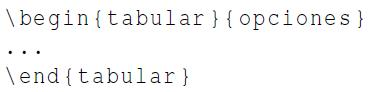
\includegraphics[scale=0.25]{SintaxisTabular.jpg}
		\end{block}
	\begin{block}{Modificadores dentro de la tabla}	
		\tiny $\backslash$hline - linea horizontal \\
		\tiny $\backslash\backslash$- Separador de filas \\
		\tiny \& - Separador de Columnas \\
		\end{block}
		

	\column {0.6\textwidth} 
		\begin{block}{Ejemplo12}			
		%\includegraphics[scale=0.40]{codigo2.jpg}
			\begin{minipage}{3cm}
% 				\testcodedoce
				\archivolatex{doce.tex}	 

	 		\end{minipage}	
		
		\end{block}
	 \end{columns}

}

%\subsection{Refere}
\frame{
	\frametitle{Referencia a Tablas en el Texto}	
	\begin{columns}
		\column {0.4\textwidth} 
	  De forma analoga para las figuras, se debe definir una etiqueta para cada tabla del texto. Es posible definir una referencia hacia esta etiqueta. 
			\begin{block}{Sintaxis}	
				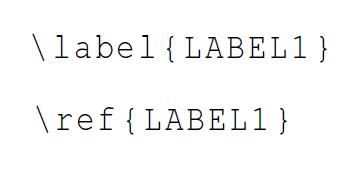
\includegraphics[scale=0.25]{Sintaxis_Label_REF.jpg}
				\end{block}
		\column {0.6\textwidth} 
		\begin{block}{Ejemplo 13}			
			\begin{minipage}{3cm}
% 				\testcodetrece
				\archivolatex{trece.tex}	 
	 		\end{minipage}			
		\end{block}
	 \end{columns}

}

%\subsection{Indice de Tablas}
\frame{
	\frametitle{Indice de Figuras y de Tablas}	
	\begin{columns}
		\column {0.4\textwidth} 
		$\backslash$listoftables y $\backslash$listoffigures se define un indice de tablas o figuras respectivamente.
		Puede ir en cualquier parte del texto
		Es poisible renombrar el nombre para adaptarlo a textos en espa\~nol. 
		\column {0.6\textwidth} 
		\begin{block}{Ejemplo 14}					
			\begin{minipage}{3cm}
% 				\testcodecatorce
				\archivolatex{catorce.tex}	 
	 		\end{minipage}			
		\end{block}
	 \end{columns}

}

\section{Referencias}
\subsection{BIBTEX}
\frame{
	\frametitle{Uso de BibTEX}		
	\begin{columns}
		\column {0.4\textwidth} 
		Se crea un archivo que se llame Biblio.bib \\
		
\begin{itemize}
	\item Este archivo contiene registros de los documentos consultados. 	
	\begin{itemize}
		\item Para cada registro debe haber una etiqueta UNICA. 
		\item Tipos de Registros: Book, Article, MasterThesis, PhDthesis, Manual
		\item \tiny Campos asociados: depende del tipo de registro
	\end{itemize}
\end{itemize}
		%Por ejemplo - Book - Necesarios: author, title, publisher y year
		%										 Opcionales: volume, series, address, edition, month.
		\column {0.6\textwidth} 
		\begin{block}{Ejemplo archivo .BIB}					
			\begin{minipage}{3cm}
				\archivolatex{quince.bib}
	 	 		\end{minipage}			
		\end{block}
	 \end{columns}
}

\subsection{BIBTEX}
\frame{
	\frametitle{Referencia en el Texto}	
	\begin{columns}
		\column {0.4\textwidth} 		
\begin{itemize}
	\item Se hace referencia a cada entrada de la lista de biblografia con $\backslash$cite\{EtiquetaEntrada\}.
	\item Con $\backslash$biblographystyle\{Tipo\}, se define el tipo de bibliografia a utilizar. Algunos otros son: amsalpha y abstract
	\item \footnotesize Con $\backslash$biblography\{NombreArchivo\}, se define el archivo (.BIB) de registros de bibliograf\'ia (Notes\'e que no se define la extensi\'on, s\'olo el nombre)
\end{itemize}
		
		\column {0.6\textwidth} 
		\begin{block}{Ejemplo 15}					
			\begin{minipage}{3cm}
% 				\testcodequince
				\archivolatex{quince.tex}

	 		\end{minipage}			
		\end{block}
	 \end{columns}

}


\frame{
	\frametitle{Generación del Archivo con Referencias Bibliográficas}	
	Se requieren la ejecución de los siguientes comandos (en ese orden el particular):
	\begin{enumerate}
		\item pdflatex NombreArchivo.tex
		\item bibtex NombreArchivo
		\item pdflatex NombreArchivo.tex
		\item pdflatex NombreArchivo.tex
	\end{enumerate}
	El comando \textbf{bibtex} obtiene información de las citas bibliográficas y genera un indice de las mismas, que es utilizado por pdflatex para el listado final.

}
\section{Ecuaciones}
\subsection{Definicion y Referencia}
\frame{
	\frametitle{Uso de Ecuaciones}
	\begin{columns}
		\column {0.4\textwidth} 
		Existen dos formas de definir ecuaciones:
		
\begin{itemize}
	\item Delimitando con los caracteres \$ \$
	\item Utilizando el entorno equation. 
	\item Superindices delimitados por \^{} y subindices delimitados por \_. 
\end{itemize}
	\begin{block}{Sintaxis}	
		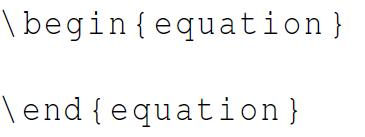
\includegraphics[scale=0.75]{Ecuacion.jpg}
	\end{block}

		\column {0.6\textwidth} 
		\begin{block}{Ejemplo 16}					
			\begin{minipage}{3cm}
				\archivolatex{dieciseis.tex}
	 		\end{minipage}			
		\end{block}
	 \end{columns}

}

\section{Integración}
\subsection{Integración}
\frame{
	\frametitle{Ejercicio}
\begin{itemize}
	\item Se necesita crear un documento con portada (con logotipos de la UPV, y diferentes tamanos de letra). Titulo de trabajo: Simulacion de Filas en SuperMercados.
	\item Tabla de contenido.
	\item Indice de figuras. 
	\item Indice de tablas.
	\item Cuatro capitulos:
		\begin{enumerate}
			\item Introduccion
			\item Teor\'ia de Colas
			\item Sistema Propuesto
			\item Resultados y Conclusiones
		\end{enumerate}
	\item \tiny Se debe incluir bibliograf\'ia de al menos 16 libros 
	\item \tiny Al menos 4 figuras y tablas por cap\'itulo
	\item \tiny Al menos 4 secciones y subsecciones por cap\'itulo
	\item \tiny Al menos 4 ecuaciones.
\end{itemize}	
}

\frame{
	%\frametitle{Ejercicio}
\begin{center}
\Huge \textbf{¡GRACIAS!}\\
\normalsize Esta presentación y los ejemplos utilizados están disponibles a peticion de quien lo solicite
\end{center}
}


\end{document}


